\documentclass[tikz]{standalone}

% \usepackage{newtxtext,newtxmath}

%!TEX root = main.tex

% mytikzset
\usepackage{tikz}
\usetikzlibrary{positioning,arrows,shapes,patterns}
\usetikzlibrary{decorations.pathmorphing}
\usetikzlibrary{decorations.markings}
\usetikzlibrary{decorations.pathreplacing}
\usetikzlibrary{calc}
\usetikzlibrary{patterns}
\usetikzlibrary{decorations.markings}
\usetikzlibrary{petri}

\tikzset{
  vector/.style={thick,double,draw=black, postaction={decorate},
    decoration={markings,mark=at position .6 with {\arrow[black,scale=0.4]{triangle 45}}}},
  axial/.style={thick,double,densely dashed,draw=black, postaction={decorate},
    decoration={markings,mark=at position .6 with {\arrow[black,scale=0.4]{triangle 45}}}},
  gluon/.style={decorate, draw=black,
    decoration={coil,aspect=0.3,segment length=5pt,amplitude=3pt}},
  pseudo/.style={thick, dashed, draw=black, postaction={decorate},
    decoration={markings,mark=at position .6 with {\arrow[red,scale=0.5]{triangle 45}}}},
  scalar/.style={thick,draw=black, postaction={decorate},
    decoration={markings,mark=at position .6 with {\arrow[black,scale=0.5]{triangle 45}}}},
  cut/.style={draw=black, decorate, decoration={snake, segment length=1mm, amplitude=0.2mm}}
}

\definecolor{myGreen}{RGB}{0,127,0}

\begin{document}
\nopagecolor
  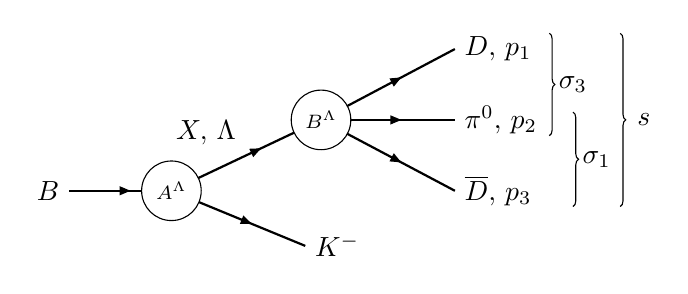
\begin{tikzpicture}[node distance=0.9cm and 1.3cm, baseline=1cm]
    \coordinate[] (c0);
    \coordinate[left=of c0,label= left:{$B$}] (Lamc);
    \coordinate[above right=of c0, xshift=6mm] (p);
    % \coordinate[below right=of c0, xshift=4mm, label=right:{$\pi^-$}] (pi);
    \coordinate[below right=of c0, xshift=4mm, yshift=2mm, label=right:{$K^-$}] (K);

    \draw[scalar]  (Lamc) --  (c0);
    \draw[scalar]  (c0) -- node[above left] {$X,\,\Lambda$} (p);
    % \draw[scalar]  (c0) -- (pi);
    \draw[scalar]  (c0) -- (K);

    \draw[black, fill=white] (c0) circle (2.5ex) node[] {\scriptsize$A^{\Lambda}$};

    \coordinate[above right=of p, xshift=4mm, label=right:{$D,\,p_1$}] (p1);
    \coordinate[      right=of p, xshift=4mm, label=right:{$\pi^0,\,p_2$}] (K1);
    \coordinate[below right=of p, xshift=4mm, label=right:{$\overline{D},\,p_3$}] (pi1);

    \draw[scalar]  (p) -- (p1);
    \draw[scalar]  (p) -- (pi1);
    \draw[scalar]  (p) -- (K1);

    \draw[black, fill=white] (p) circle (2.5ex) node[] {\scriptsize$B^{\Lambda}$};

    \draw[decorate,decoration={brace,amplitude=2pt}]
      ([xshift=+1.2cm,yshift=+.2cm]p1) -- ([xshift=+1.2cm,yshift=-.2cm]K1)
      node [black,midway,xshift=0.3cm] { $\sigma_3$};
    \draw[decorate,decoration={brace,amplitude=2pt}]
      ([xshift=+1.5cm,yshift=+.1cm]K1) -- ([xshift=+1.5cm,yshift=-.2cm]pi1)
      node [black,midway,xshift=0.3cm] { $\sigma_1$};
    \draw[decorate,decoration={brace,amplitude=2pt}]
      ([xshift=+2.1cm,yshift=+.2cm]p1) -- ([xshift=+2.1cm,yshift=-.2cm]pi1)
      node [black,midway,xshift=0.3cm] {$s$};
  \end{tikzpicture}
\end{document}
